    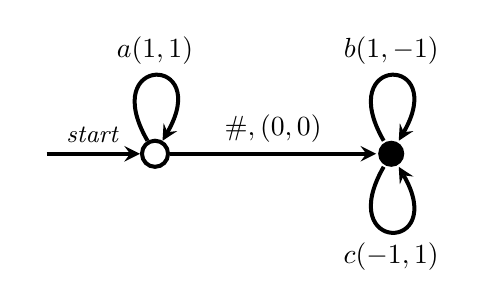
\begin{tikzpicture}
        \node (qs) at (-1.5, 0) {};
        \node[draw, circle, minimum size = 0.1in, line width = 0.02in] (q1) at (0,0) {};
        \node[fill, circle, minimum size = 0.1in, line width = 0.02in] (qf) at (3,0) {};

        \draw[-stealth, line width = 0.02in] (qs) -- node[above] {\small\textit{start}} (q1);
        
        \draw[-stealth, line width = 0.02in] (q1) edge[loop above, distance = 0.5in, out=120, in=60] node[above] {$a(1, 1)$} (q1);
        
        \draw[-stealth, line width = 0.02in] (q1) -- node[above] {$\#, (0, 0)$} (qf);
        
        \draw[-stealth, line width = 0.02in] (qf) edge[loop above, distance = 0.5in, out=120, in=60] node[above] {$b(1, -1)$} (qf);
        \draw[-stealth, line width = 0.02in] (qf) edge[loop below, distance = 0.5in, out=240, in=300] node[below] {$c(-1, 1)$} (qf);
\end{tikzpicture}